\documentclass{article}

% content/resources/templates/preamble.tex
\usepackage[margin=0.6in]{geometry}
\author{Milav Dabgar}
\usepackage{amsmath,amssymb,amsthm}
\usepackage{booktabs}
\usepackage{multirow}
\usepackage{xcolor}
\usepackage{tcolorbox}
\tcbuselibrary{breakable,skins}
\usepackage[colorlinks=true,linkcolor=blue]{hyperref}
\usepackage{titlesec}
\usepackage{enumitem}
\usepackage{tikz}
\usepackage{pgfplots}
\usepackage{circuitikz}
\usepackage[version=4]{mhchem}
\usepackage{longtable}
\usepackage{array}
\usepackage{float}
\usepackage{caption}
\usepackage{listings}

\lstset{
  basicstyle=\small\ttfamily,
  breaklines=true,
  breakatwhitespace=false,
  postbreak=\mbox{\textcolor{red}{$\hookrightarrow$}\space},
  float=false,
  numbers=left,
  numberstyle=\tiny\color{gray},
  numbersep=10pt,
  xleftmargin=2em,
  keywordstyle=\color{blue},
  commentstyle=\color{green!60!black},
  stringstyle=\color{purple},
  backgroundcolor=\color{gray!5},
  showstringspaces=false,
  tabsize=2,
  captionpos=b,
  keepspaces=true,
  columns=flexible
}

\pgfplotsset{compat=1.18}
\usetikzlibrary{shapes,arrows,positioning,calc,patterns,decorations.pathmorphing,decorations.markings,arrows.meta}

% Color scheme
\definecolor{headcolor}{RGB}{0,102,204}
\definecolor{keycolor}{RGB}{220,20,60}
\definecolor{solutioncolor}{RGB}{34,139,34}
\definecolor{mnemoniccolor}{RGB}{148,0,211}
\definecolor{codecolor}{RGB}{0,0,100}

% Spacing
\setlength{\parskip}{3pt}
\setlist[itemize]{nosep}
\setlist[enumerate]{nosep}

% Title formatting
\titleformat{\section}{\Large\bfseries\color{headcolor}}{\thesection}{1em}{}
\titleformat{\subsection}{\large\bfseries\color{headcolor}}{\thesubsection}{1em}{}

% Pandoc tightlist compatibility
\providecommand{\tightlist}{%
  \setlength{\itemsep}{0pt}\setlength{\parskip}{0pt}}

% Pandoc longtable compatibility
\newcounter{none}
\def\thenone{}


% content/resources/templates/english-boxes.tex

% Custom environments
\newtcolorbox{solutionbox}{
 breakable,
 enhanced,
 colback=solutioncolor!5!white,
 colframe=solutioncolor!75!black,
 fonttitle=\bfseries,
 title=Solution
}

\newtcolorbox{solutionboxnobreak}{
 colback=solutioncolor!5!white,
 colframe=solutioncolor!75!black,
 fonttitle=\bfseries,
 title=Solution
}

\newtcolorbox{keyformula}{
 breakable,
 enhanced,
 colback=keycolor!5!white,
 colframe=keycolor!75!black,
 fonttitle=\bfseries,
 title=Key Formula
}

\newtcolorbox{mnemonicboxenv}{
 breakable,
 enhanced,
 colback=mnemoniccolor!5!white,
 colframe=mnemoniccolor!75!black,
 fonttitle=\bfseries,
 title=Mnemonic
}

\newcommand{\mnemonicbox}[1]{%
  \begin{mnemonicboxenv}
    #1
  \end{mnemonicboxenv}
}


% Custom commands for GTU solutions
% This file defines semantic commands for consistent formatting

% Question command with automatic formatting
\newcommand{\question}[2]{%
  \section*{Question #1}%
  \textbf{#2}%
}

% OR question variant
\newcommand{\questionor}[2]{%
  \section*{Question #1 OR}%
  \textbf{#2}%
}

% Proper table environment with caption
\newenvironment{answertable}[1]{%
  \begin{table}[htbp]
  \centering
  \caption{#1}
}{%
  \end{table}
}

% Proper figure environment for diagrams
\newenvironment{answerdiagram}[1]{%
  \begin{figure}[htbp]
  \centering
  \caption{#1}
}{%
  \end{figure}
}

% Semantic markup for key terms
\newcommand{\keyword}[1]{\textbf{#1}}
\newcommand{\code}[1]{\texttt{#1}}
\newcommand{\classname}[1]{\texttt{#1}}
\newcommand{\methodname}[1]{\texttt{#1}}

% Proper quotation marks
\newcommand{\mnemonic}[1]{``#1''}


\title{Communication Engineering (1333201) - Winter 2023 Solution}
\date{January 11, 2024}

\begin{document}
\maketitle

\questionmarks{1(a)}{3}{Define: (A) Amplitude Modulation, (B) Frequency Modulation, and (C) Phase Modulation}

\begin{solutionbox}
\textbf{Answer}:

\begin{center}
\captionof{table}{Types of Modulation Techniques}
\begin{tabulary}{\linewidth}{|L|L|}
\hline
\textbf{Modulation Type} & \textbf{Definition} \\
\hline
\textbf{Amplitude Modulation (AM)} & Process where amplitude of carrier signal is varied according to the instantaneous value of modulating signal while frequency remains constant \\
\hline
\textbf{Frequency Modulation (FM)} & Process where frequency of carrier signal is varied according to the instantaneous value of modulating signal while amplitude remains constant \\
\hline
\textbf{Phase Modulation (PM)} & Process where phase of carrier signal is varied according to the instantaneous value of modulating signal while amplitude remains constant \\
\hline
\end{tabulary}
\end{center}
\end{solutionbox}

\begin{mnemonicbox}
"A-F-P: Amplitude changes, Frequency shifts, Phase adjusts"
\end{mnemonicbox}

\questionmarks{1(b)}{4}{Explain the need for modulation.}

\begin{solutionbox}
\textbf{Answer}:

\begin{center}
\captionof{table}{Need for Modulation}
\begin{tabulary}{\linewidth}{|L|L|}
\hline
\textbf{Need} & \textbf{Explanation} \\
\hline
\textbf{Practical Antenna Size} & Reduces antenna size by increasing frequency (Antenna length = $\lambda/4$) \\
\hline
\textbf{Interference Reduction} & Allows multiple signals to be transmitted simultaneously on different frequencies \\
\hline
\textbf{Range Extension} & Higher frequency signals travel farther in atmosphere \\
\hline
\textbf{Multiplexing} & Enables multiple signals to share communication medium \\
\hline
\end{tabulary}
\end{center}

\begin{center}
\begin{tikzpicture}[auto, >=latex, thick]
    \node [gtu block] (need) {Need for Modulation};
    \node [gtu block, below of=need, node distance=2cm, xshift=-4.5cm] (size) {Practical\\Antenna Size};
    \node [gtu block, below of=need, node distance=2cm, xshift=-1.5cm] (inter) {Interference\\Reduction};
    \node [gtu block, below of=need, node distance=2cm, xshift=1.5cm] (range) {Range\\Extension};
    \node [gtu block, below of=need, node distance=2cm, xshift=4.5cm] (mux) {Multiplexing};
    
    \draw [gtu arrow] (need) -- (size);
    \draw [gtu arrow] (need) -- (inter);
    \draw [gtu arrow] (need) -- (range);
    \draw [gtu arrow] (need) -- (mux);
\end{tikzpicture}
\captionof{figure}{Need for Modulation}
\end{center}
\end{solutionbox}

\begin{mnemonicbox}
"PIRM: Practical antennas, Interference reduction, Range extension, Multiplexing"
\end{mnemonicbox}

\questionmarks{1(c)}{7}{A modulating signal has amplitude of 3 V and frequency of 1 KHz is amplitude modulated by a carrier of amplitude 10 V and frequency 30KHz. Find modulation index, frequencies of sideband components and their amplitudes. Also draw the spectrum of AM wave.}

\begin{solutionbox}
\textbf{Answer}:

\textbf{Given Information:}
\begin{itemize}
    \item Modulating Signal: $A_m = 3$ V, $f_m = 1$ kHz
    \item Carrier Signal: $A_c = 10$ V, $f_c = 30$ kHz
\end{itemize}

\textbf{Calculations:}

\begin{enumerate}
    \item \textbf{Modulation Index (m)}:
    \[ m = \frac{A_m}{A_c} = \frac{3}{10} = 0.3 \]
    
    \item \textbf{Sideband Frequencies}:
    \[ f_{LSB} = f_c - f_m = 30 - 1 = 29 \text{ kHz} \]
    \[ f_{USB} = f_c + f_m = 30 + 1 = 31 \text{ kHz} \]
    
    \item \textbf{Sideband Amplitudes}:
    \[ A_{SB} = \frac{m \cdot A_c}{2} = \frac{0.3 \cdot 10}{2} = 1.5 \text{ V} \]
\end{enumerate}

\begin{center}
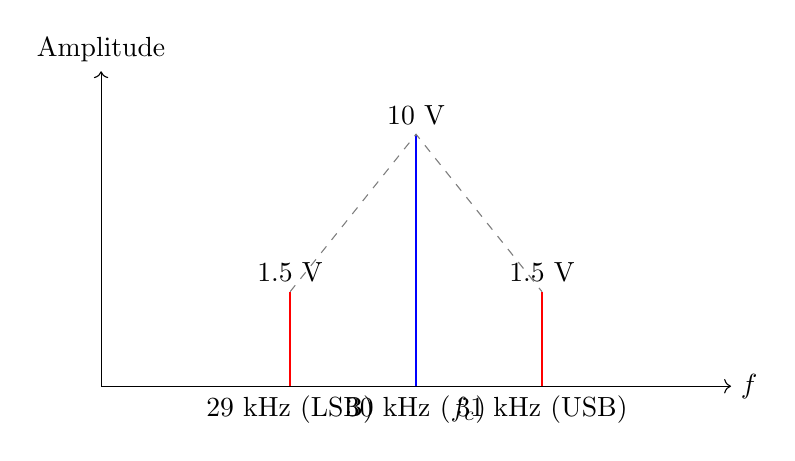
\begin{tikzpicture}[scale=0.8]
    \draw[->] (0,0) -- (10,0) node[right] {$f$};
    \draw[->] (0,0) -- (0,5) node[above] {Amplitude};
    
    % Carrier
    \draw[thick, blue] (5,0) -- (5,4);
    \node[above] at (5,4) {10 V};
    \node[below] at (5,0) {30 kHz ($f_c$)};
    
    % LSB
    \draw[thick, red] (3,0) -- (3,1.5);
    \node[above] at (3,1.5) {1.5 V};
    \node[below] at (3,0) {29 kHz (LSB)};
    
    % USB
    \draw[thick, red] (7,0) -- (7,1.5);
    \node[above] at (7,1.5) {1.5 V};
    \node[below] at (7,0) {31 kHz (USB)};
    
    % connecting lines (envelope shape hint)
    \draw[dashed, gray] (3,1.5) -- (5,4) -- (7,1.5);
\end{tikzpicture}
\captionof{figure}{AM Spectrum}
\end{center}
\end{solutionbox}

\begin{mnemonicbox}
"LSB-C-USB: Lower sideband, Carrier, Upper sideband at 29-30-31"
\end{mnemonicbox}

\questionmarks{1(c) OR}{7}{Derive mathematical relation between carrier powers, and modulated signal power for AM.}

\begin{solutionbox}
\textbf{Answer}:

\textbf{Mathematical Relation:}

Only the carrier signal is: $c(t) = A_c \cos(2\pi f_c t)$
The modulating signal is: $m(t) = A_m \cos(2\pi f_m t)$
The AM signal equation is:
\[ s(t) = A_c [1 + m \cos(2\pi f_m t)] \cos(2\pi f_c t) \]
Expanding this:
\[ s(t) = A_c \cos(2\pi f_c t) + \frac{m A_c}{2} \cos[2\pi(f_c - f_m)t] + \frac{m A_c}{2} \cos[2\pi(f_c + f_m)t] \]

\textbf{Power Calculations:}
Power is proportional to square of amplitude ($P = V^2/R$, assuming R=1$\Omega$).

1. \textbf{Carrier Power ($P_c$)}:
\[ P_c = \frac{(A_c/\sqrt{2})^2}{R} = \frac{A_c^2}{2} \]

2. \textbf{Total Sideband Power ($P_s$)}:
\[ P_{LSB} = \frac{(m A_c/2\sqrt{2})^2}{R} = \frac{m^2 A_c^2}{8} \]
\[ P_{USB} = \frac{(m A_c/2\sqrt{2})^2}{R} = \frac{m^2 A_c^2}{8} \]
\[ P_s = P_{LSB} + P_{USB} = \frac{m^2 A_c^2}{4} = P_c \cdot \frac{m^2}{2} \]

3. \textbf{Total AM Power ($P_t$)}:
\[ P_t = P_c + P_s = P_c + P_c \frac{m^2}{2} \]
\[ P_t = P_c \left( 1 + \frac{m^2}{2} \right) \]

\begin{center}
\captionof{table}{Power Distribution in AM}
\begin{tabulary}{\linewidth}{|L|L|L|}
\hline
\textbf{Component} & \textbf{Expression} & \textbf{In Terms of $P_c$} \\
\hline
\textbf{Carrier Power ($P_c$)} & $A_c^2/2$ & $P_c$ \\
\hline
\textbf{Total Sideband Power ($P_s$)} & $m^2 A_c^2/4$ & $m^2 P_c/2$ \\
\hline
\textbf{Total AM Power ($P_t$)} & $P_c(1 + m^2/2)$ & $P_c(1 + m^2/2)$ \\
\hline
\end{tabulary}
\end{center}

\textbf{Modulation Efficiency ($\eta$)}: ratio of sideband power to total power.
\[ \eta = \frac{P_s}{P_t} = \frac{m^2/2}{1 + m^2/2} \times 100\% \]
For 100\% modulation ($m=1$), $\eta = 33.3\%$.
\end{solutionbox}

\begin{mnemonicbox}
"Total Power = Carrier Power × (1 + m²/2)"
\end{mnemonicbox}

\questionmarks{2(a)}{3}{Compare AM and FM.}

\begin{solutionbox}
\textbf{Answer}:

\begin{center}
\captionof{table}{Comparison between AM and FM}
\begin{tabulary}{\linewidth}{|L|L|L|}
\hline
\textbf{Parameter} & \textbf{AM} & \textbf{FM} \\
\hline
\textbf{Modulation Parameter} & Amplitude varies & Frequency varies \\
\hline
\textbf{Bandwidth} & $2 \times f_m$ & $2 \times (\Delta f + f_m)$ \\
\hline
\textbf{Noise Immunity} & Poor & Excellent \\
\hline
\textbf{Power Efficiency} & Low & High \\
\hline
\textbf{Circuit Complexity} & Simple & Complex \\
\hline
\end{tabulary}
\end{center}
\end{solutionbox}

\begin{mnemonicbox}
"ABNPC: Amplitude/Bandwidth/Noise/Power/Complexity differences"
\end{mnemonicbox}

\questionmarks{2(b)}{4}{Explain envelope detector with the help of circuit diagram.}

\begin{solutionbox}
\textbf{Answer}:

\begin{center}
\begin{tikzpicture}[auto, >=latex, thick]
    \node (input) {AM Input};
    \node [draw, circle, right of=input, node distance=2.5cm, inner sep=0pt] (diode) {};
    \node [right of=diode, node distance=0.5cm] {}; 
    % Standard Diode symbol is tricky in pure nodes, using standard drawing
    
    \draw [gtu arrow] (input) -- (1,0);
    \draw [thick] (1.5, -0.5) -- (1.5, 0.5) -- (2.5, 0) -- cycle; % Diode triangle
    \draw [thick] (2.5, -0.5) -- (2.5, 0.5); % Diode bar
    \draw [thick] (2.5, 0) -- (4, 0);
    
    % RC Network
    \draw [thick] (4,0) -- (4,-2);
    \draw [thick] (3.5, 0) -- (3.5, -0.8);
    \draw [thick] (3, -0.8) -- (4, -0.8); % Capacitor top
    \draw [thick] (3, -1.2) -- (4, -1.2); % Capacitor bottom
    \draw [thick] (3.5, -1.2) -- (3.5, -2);
    
    % Resistor
    \draw [thick] (5.5, 0) -- (5.5, -0.5) -- (5.7, -0.7) -- (5.3, -0.9) -- (5.7, -1.1) -- (5.3, -1.3) -- (5.5, -1.5) -- (5.5, -2);
    
    \draw [thick] (3.5, -2) -- (5.5, -2);
    \draw [thick] (4,0) -- (6.5, 0);
    \node [right] at (6.5, 0) {Output};
    
    % Labels
    \node [above] at (2, 0.5) {Diode (D)};
    \node [left] at (3, -1) {C};
    \node [right] at (5.7, -1) {R};
\end{tikzpicture}
% Let's use a cleaner TikZ for Envelope Detector
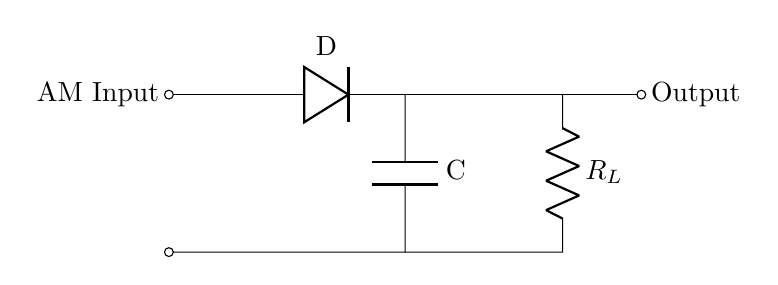
\begin{tikzpicture}[scale=1]
    \draw (0,0) to[short, o-] (1,0) 
        to[diode, l=D] (3,0) -- (5,0)
        to[short, -o] (6,0) node[right] {Output};
    
    \draw (3,0) to[C, l=C] (3,-2) -- (0,-2) to[short, -o] (0,-2);
    \draw (5,0) to[R, l=$R_L$] (5,-2) -- (3,-2);
    
    \node[left] at (0,0) {AM Input};
\end{tikzpicture}
% Wait, standard LaTeX doesn't have circuitikz loaded by default in our template probably.
% Reverting to standard TikZ shapes.
\nopagebreak
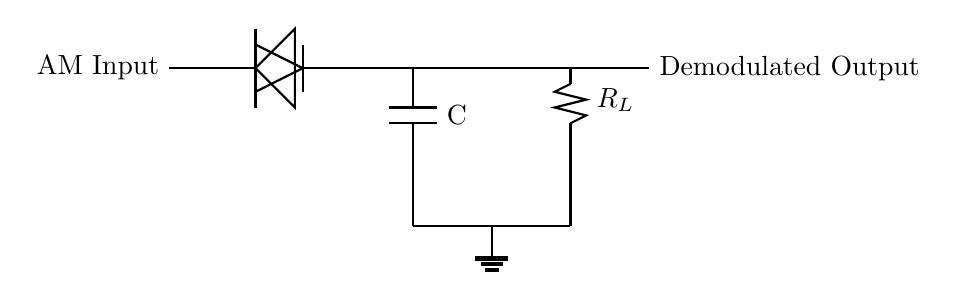
\begin{tikzpicture}[auto, >=latex, thick]
   \node (in) at (0,2) {AM Input};
   \draw (in) -- (2,2);
   
   % Diode
   \draw (2,2) -- (2.5,2.5) -- (2.5,1.5) -- (2,2); % Triangle pointing left? No pointing right
   \draw (2,2.5) -- (2,1.5); % Wait, triangle points to bar. Input is anode.
   % Correct Diode:
   \draw[thick] (2,2) -- (2,2); % Wire
   \draw[thick] (2,2.3) -- (2,1.7) -- (2.6,2) -- cycle; % Triangle
   \draw[thick] (2.6,2.3) -- (2.6,1.7); % Bar
   \draw[thick] (2.6,2) -- (4,2);
   
   % Capacitor
   \draw[thick] (4,2) -- (4,1.5);
   \draw[thick] (3.7,1.5) -- (4.3,1.5);
   \draw[thick] (3.7,1.3) -- (4.3,1.3);
   \draw[thick] (4,1.3) -- (4,0);
   \node[right] at (4.3,1.4) {C};
   
   % Resistor
   \draw[thick] (6,2) -- (6,1.8);
   \draw[thick] (6,1.8) -- (5.8,1.7) -- (6.2,1.6) -- (5.8,1.5) -- (6.2,1.4) -- (6,1.3);
   \draw[thick] (6,1.3) -- (6,0);
   \node[right] at (6.2,1.6) {$R_L$};
   
   % Connections
   \draw[thick] (4,2) -- (7,2);
   \node[right] at (7,2) {Demodulated Output};
   \draw[thick] (4,0) -- (6,0); % Ground line
   \node[ground] at (5,0) {};
\end{tikzpicture}
\captionof{figure}{Envelope Detector Circuit}
\end{center}

\textbf{Envelope Detector Components:}

\begin{center}
\captionof{table}{Component Functions}
\begin{tabulary}{\linewidth}{|L|L|}
\hline
\textbf{Component} & \textbf{Function} \\
\hline
\textbf{Diode (D)} & Rectifies AM signal to extract positive half cycles \\
\hline
\textbf{Capacitor (C)} & Charges to peak of input, holds charge between peaks \\
\hline
\textbf{Resistor ($R_L$)} & Discharges capacitor at rate suitable for envelope extraction \\
\hline
\end{tabulary}
\end{center}

\textbf{Time Constant Selection:}
\[ \frac{1}{f_c} \ll RC \ll \frac{1}{f_m} \]
(Correct standard condition for proper envelope detection)
\end{solutionbox}

\begin{mnemonicbox}
"DCR: Diode rectifies, Capacitor charges, Resistor discharges"
\end{mnemonicbox}

\questionmarks{2(c)}{7}{Draw and explain the block diagram of Superheterodyne receiver.}

\begin{solutionbox}
\textbf{Answer}:

\begin{center}
\begin{tikzpicture}[node distance=2.5cm, auto, >=latex, thick, scale=0.8, transform shape]
    \node [gtu block] (rf) {RF\\Amplifier};
    \node [left of=rf, node distance=2.5cm] (ant) {Antenna};
    \node [gtu block, right of=rf] (mix) {Mixer};
    \node [gtu block, below of=mix] (lo) {Local\\Oscillator};
    \node [gtu block, right of=mix] (if) {IF\\Amplifier};
    \node [gtu block, right of=if] (det) {Detector};
    \node [gtu block, right of=det] (af) {AF\\Amplifier};
    \node [right of=af, node distance=2.5cm] (spk) {Speaker};
    
    \draw [gtu arrow] (ant) -- (rf);
    \draw [gtu arrow] (rf) -- (mix);
    \draw [gtu arrow] (lo) -- (mix);
    \draw [gtu arrow] (mix) -- (if);
    \draw [gtu arrow] (if) -- (det);
    \draw [gtu arrow] (det) -- (af);
    \draw [gtu arrow] (af) -- (spk);
\end{tikzpicture}
\captionof{figure}{Superheterodyne Receiver}
\end{center}

\textbf{Functions of Blocks:}

\begin{center}
\captionof{table}{Receiver Blocks}
\begin{tabulary}{\linewidth}{|L|L|}
\hline
\textbf{Block} & \textbf{Function} \\
\hline
\textbf{RF Amplifier} & Amplifies weak RF signal, provides selectivity, rejects image frequency \\
\hline
\textbf{Local Oscillator} & Generates frequency $f_o = f_{RF} + f_{IF}$ for mixing \\
\hline
\textbf{Mixer} & Combines RF signal with local oscillator to produce IF (Intermediate Frequency) \\
\hline
\textbf{IF Amplifier} & Provides most of the receiver gain and selectivity at fixed frequency \\
\hline
\textbf{Detector} & Extracts the modulating signal from the IF signal \\
\hline
\textbf{AF Amplifier} & Amplifies recovered audio to drive speaker \\
\hline
\end{tabulary}
\end{center}
\end{solutionbox}

\begin{mnemonicbox}
"RLMIDS: RF, Local oscillator, Mixer, IF, Detector, Speaker"
\end{mnemonicbox}

\questionmarks{2(a) OR}{3}{Define the followings terms: (A) Sensitivity, and (B) Selectivity}

\begin{solutionbox}
\textbf{Answer}:

\begin{center}
\captionof{table}{Receiver Characteristics}
\begin{tabulary}{\linewidth}{|L|L|}
\hline
\textbf{Term} & \textbf{Definition} \\
\hline
\textbf{Sensitivity} & Ability of receiver to detect and amplify weak signals; measured as minimum input signal strength ($\mu$V) needed for standard output \\
\hline
\textbf{Selectivity} & Ability of receiver to separate desired signal from adjacent channels; measured as ratio of response at resonant frequency to off-resonant frequency \\
\hline
\end{tabulary}
\end{center}

\begin{center}
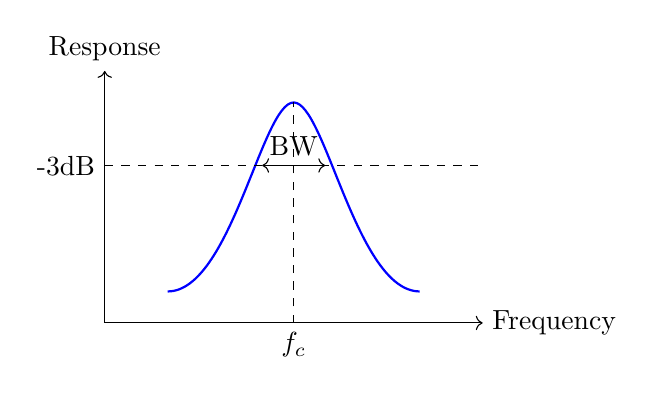
\begin{tikzpicture}[scale=0.8]
    \draw[->] (0,0) -- (6,0) node[right] {Frequency};
    \draw[->] (0,0) -- (0,4) node[above] {Response};
    
    % Selectivity Curve
    \draw[thick, blue] (1,0.5) .. controls (2,0.5) and (2.5,3.5) .. (3,3.5) 
                       .. controls (3.5,3.5) and (4,0.5) .. (5,0.5);
    
    \draw[dashed] (3,0) -- (3,3.5);
    \node[below] at (3,0) {$f_c$};
    
    \draw[dashed] (0, 2.5) -- (6, 2.5);
    \node[left] at (0, 2.5) {-3dB};
    
    \draw[<->] (2.5, 2.5) -- (3.5, 2.5);
    \node[above] at (3, 2.5) {BW};
\end{tikzpicture}
\captionof{figure}{Selectivity Curve}
\end{center}
\end{solutionbox}

\begin{mnemonicbox}
"SS: Signal Strength for Sensitivity, Signal Separation for Selectivity"
\end{mnemonicbox}

\questionmarks{2(b) OR}{4}{Describe the block diagram of general communication system.}

\begin{solutionbox}
\textbf{Answer}:

\begin{center}
\begin{tikzpicture}[node distance=2.5cm, auto, >=latex, thick]
    \node [gtu block] (source) {Information\\Source};
    \node [gtu block, right of=source, node distance=3cm] (tx) {Transmitter};
    \node [gtu block, right of=tx, node distance=3cm] (ch) {Channel};
    \node [gtu block, right of=ch, node distance=3cm] (rx) {Receiver};
    \node [gtu block, right of=rx, node distance=3cm] (dest) {Destination};
    \node [gtu block, below of=ch, node distance=2cm] (noise) {Noise\\Source};
    
    \draw [gtu arrow] (source) -- (tx);
    \draw [gtu arrow] (tx) -- (ch);
    \draw [gtu arrow] (ch) -- (rx);
    \draw [gtu arrow] (rx) -- (dest);
    \draw [gtu arrow] (noise) -- (ch);
\end{tikzpicture}
\captionof{figure}{General Communication System}
\end{center}

\begin{center}
\captionof{table}{Components of Communication System}
\begin{tabulary}{\linewidth}{|L|L|}
\hline
\textbf{Component} & \textbf{Function} \\
\hline
\textbf{Information Source} & Generates message to be communicated (voice, data, video) \\
\hline
\textbf{Transmitter} & Converts message into signals suitable for transmission \\
\hline
\textbf{Channel} & Medium through which signals travel (wire, fiber, air) \\
\hline
\textbf{Receiver} & Extracts original message from received signals \\
\hline
\textbf{Destination} & Entity for which message is intended \\
\hline
\textbf{Noise Source} & Unwanted signals that interfere with the message \\
\hline
\end{tabulary}
\end{center}
\end{solutionbox}

\begin{mnemonicbox}
"I-T-C-R-D: Information Travels Carefully, Reaches Destination"
\end{mnemonicbox}

\questionmarks{2(c) OR}{7}{Draw and explain the block diagram of Superheterodyne FM receiver.}

\begin{solutionbox}
\textbf{Answer}:

\begin{center}
\begin{tikzpicture}[node distance=2.2cm, auto, >=latex, thick, scale=0.75, transform shape]
    \node [gtu block] (rf) {RF\\Amp};
    \node [left of=rf, node distance=2cm] (ant) {Ant};
    \node [gtu block, right of=rf] (mix) {Mixer};
    \node [gtu block, below of=mix] (lo) {Local\\Osc};
    \node [gtu block, right of=mix] (if) {IF\\Amp};
    \node [gtu block, right of=if] (lim) {Limiter};
    \node [gtu block, right of=lim] (disc) {FM\\Discrim.};
    \node [gtu block, right of=disc] (deemp) {De-\\emphasis};
    \node [gtu block, right of=deemp] (af) {AF\\Amp};
    \node [right of=af, node distance=2cm] (spk) {Spk};
    
    \draw [gtu arrow] (ant) -- (rf);
    \draw [gtu arrow] (rf) -- (mix);
    \draw [gtu arrow] (lo) -- (mix);
    \draw [gtu arrow] (mix) -- (if);
    \draw [gtu arrow] (if) -- (lim);
    \draw [gtu arrow] (lim) -- (disc);
    \draw [gtu arrow] (disc) -- (deemp);
    \draw [gtu arrow] (deemp) -- (af);
    \draw [gtu arrow] (af) -- (spk);
\end{tikzpicture}
\captionof{figure}{Superheterodyne FM Receiver}
\end{center}

\textbf{Additional Components in FM Receiver:}

\begin{center}
\captionof{table}{FM Specific Components}
\begin{tabulary}{\linewidth}{|L|L|}
\hline
\textbf{Component} & \textbf{Function} \\
\hline
\textbf{Limiter} & Removes amplitude variations, provides constant amplitude signal \\
\hline
\textbf{FM Discriminator} & Converts frequency variations to amplitude variations (demodulation) \\
\hline
\textbf{De-emphasis} & Attenuates higher frequencies boosted at transmitter \\
\hline
\end{tabulary}
\end{center}

\textbf{Unique Aspects of FM Receiver:}
\begin{itemize}
    \item Uses wider bandwidth IF amplifier (200 kHz vs 10 kHz for AM)
    \item Requires limiter stage for noise reduction
    \item Employs specialized discriminator for FM demodulation
\end{itemize}
\end{solutionbox}

\begin{mnemonicbox}
"MILD: Mixer, IF, Limiter, Discriminator - key components in FM reception"
\end{mnemonicbox}

\questionmarks{3(a)}{3}{What is PAM?}

\begin{solutionbox}
\textbf{Answer}:

\textbf{Pulse Amplitude Modulation (PAM):}
PAM is a modulation technique where the amplitude of regularly spaced rectangular pulses allows variation according to the instantaneous value of the modulating signal.

\begin{itemize}
    \item \textbf{Process}: Analog signal is sampled at regular intervals.
    \item \textbf{Result}: A train of pulses where pulse height $\propto$ signal amplitude.
    \item \textbf{Types}: Natural sampling, Flat-top sampling.
\end{itemize}

\begin{center}
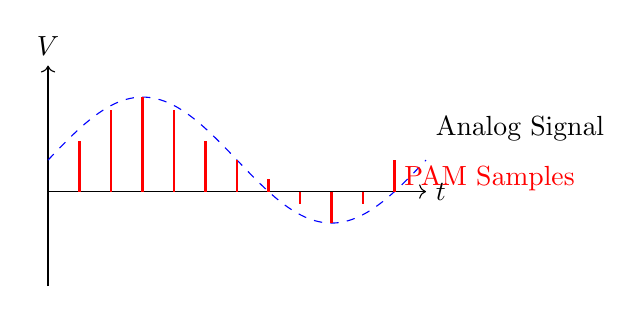
\begin{tikzpicture}[scale=0.8]
    \draw[->] (0,0) -- (6,0) node[right] {$t$};
    \draw[->] (0,-1.5) -- (0,2) node[above] {$V$};
    
    % Analog envelope
    \draw[dashed, blue] (0,0.5) sin (1.5,1.5) cos (3,0.5) sin (4.5,-0.5) cos (6,0.5);
    
    % PAM Pulses
    \foreach \x/\y in {0.5/0.8, 1.0/1.3, 1.5/1.5, 2.0/1.3, 2.5/0.8, 3.0/0.5, 3.5/0.2, 4.0/-0.2, 4.5/-0.5, 5.0/-0.2, 5.5/0.5}
        \draw[thick, red] (\x,0) -- (\x,\y);
        
    \node[right] at (6,1) {Analog Signal};
    \node[right, red] at (5.5, 0.2) {PAM Samples};
\end{tikzpicture}
\captionof{figure}{PAM Waveform}
\end{center}
\end{solutionbox}

\begin{mnemonicbox}
"PAM: Pulse Amplitude Matches signal"
\end{mnemonicbox}

\questionmarks{3(b)}{4}{State and prove sampling theorem.}

\begin{solutionbox}
\textbf{Answer}:

\textbf{Statement:}
A continuous-time signal $x(t)$ with maximum frequency $f_m$ can be completely reconstructed from its samples if the sampling frequency $f_s$ satisfies:
\[ f_s \ge 2 f_m \]
Where $2 f_m$ is called the Nyquist rate.

\textbf{Proof (Conceptual):}
Consider a signal $x(t)$ with spectrum $X(f)$ band-limited to $f_m$.

1.  \textbf{Sampling Process}: Sampling is equivalent to multiplying $x(t)$ by a pulse train $\delta(t)$.
2.  \textbf{Frequency Domain}: Multiplication in time is convolution in frequency.
    \[ X_s(f) = f_s \sum_{n=-\infty}^{\infty} X(f - n f_s) \]
3.  \textbf{Spectrum Replication}: The spectrum of sampled signal consists of replicas of $X(f)$ spaced at intervals of $f_s$.
4.  \textbf{Recovery Condition}: To recover original spectrum without overlap (aliasing):
    \[ f_s - f_m \ge f_m \implies f_s \ge 2 f_m \]

\begin{center}
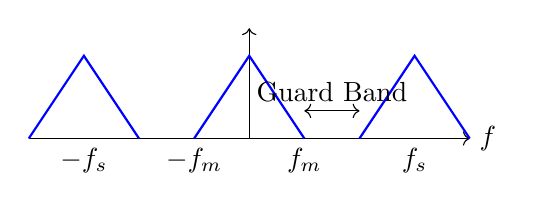
\begin{tikzpicture}[scale=0.7]
    \draw[->] (-4,0) -- (4,0) node[right] {$f$};
    \draw[->] (0,0) -- (0,2);
    
    % Baseband
    \draw[thick, blue] (-1,0) -- (0,1.5) -- (1,0);
    \node[below] at (1,0) {$f_m$};
    \node[below] at (-1,0) {$-f_m$};
    
    % Replicas
    \draw[thick, blue] (2,0) -- (3,1.5) -- (4,0);
    \node[below] at (3,0) {$f_s$};
    \draw[thick, blue] (-4,0) -- (-3,1.5) -- (-2,0);
    \node[below] at (-3,0) {$-f_s$};
    
    \draw[<->] (1,0.5) -- (2,0.5);
    \node[above] at (1.5,0.5) {Guard Band};
\end{tikzpicture}
\captionof{figure}{Sampled Signal Spectrum ($f_s > 2f_m$)}
\end{center}
\end{solutionbox}

\begin{mnemonicbox}
"Nyquist: Sample twice the max frequency to avoid aliasing"
\end{mnemonicbox}

\questionmarks{3(c)}{7}{Draw and Explain block diagram of digital communication system.}

\begin{solutionbox}
\textbf{Answer}:

\begin{center}
\begin{tikzpicture}[node distance=2.2cm, auto, >=latex, thick, scale=0.7, transform shape]
    % Transmitter
    \node [gtu block] (source) {Source};
    \node [gtu block, right of=source] (fmt) {Source\\Encoder};
    \node [gtu block, right of=fmt] (ch) {Channel\\Encoder};
    \node [gtu block, right of=ch] (mod) {Digital\\Modulator};
    
    % Channel
    \node [gtu block, below of=mod, node distance=2cm] (chan) {Channel};
    
    % Receiver
    \node [gtu block, left of=chan] (demod) {Digital\\Demodulator};
    \node [gtu block, left of=demod] (chd) {Channel\\Decoder};
    \node [gtu block, left of=chd] (fmd) {Source\\Decoder};
    \node [gtu block, left of=fmd] (dest) {User};
    
    \draw [gtu arrow] (source) -- (fmt);
    \draw [gtu arrow] (fmt) -- (ch);
    \draw [gtu arrow] (ch) -- (mod);
    \draw [gtu arrow] (mod) -- (chan);
    \draw [gtu arrow] (chan) -- (demod);
    \draw [gtu arrow] (demod) -- (chd);
    \draw [gtu arrow] (chd) -- (fmd);
    \draw [gtu arrow] (fmd) -- (dest);
\end{tikzpicture}
\captionof{figure}{Digital Communication System}
\end{center}

\begin{center}
\captionof{table}{Functions of Blocks}
\begin{tabulary}{\linewidth}{|L|L|}
\hline
\textbf{Block} & \textbf{Function} \\
\hline
\textbf{Source Encoder} & Removes redundancy to compress data / converts analog to digital (ADC) \\
\hline
\textbf{Channel Encoder} & Adds redundancy bits for error detection and correction \\
\hline
\textbf{Digital Modulator} & Converts digital bits into analog waveform (ASK, FSK, PSK) suitable for channel \\
\hline
\textbf{Channel} & Transmission medium, adds noise and interference \\
\hline
\textbf{Digital Demodulator} & Estimates Transmitted bits from received noisy waveform \\
\hline
\textbf{Channel Decoder} & Uses redundancy to detect/correct errors \\
\hline
\textbf{Source Decoder} & Reconstructs original information from bits \\
\hline
\end{tabulary}
\end{center}
\end{solutionbox}

\begin{mnemonicbox}
"S-C-M-C-D-C-S: Source, Channel, Modulate, Channel, Demodulate, Decode, Sink"
\end{mnemonicbox}

\questionmarks{3(a) OR}{3}{What is PWM?}

\begin{solutionbox}
\textbf{Answer}:

\textbf{Pulse Width Modulation (PWM):}
PWM (also known as Pulse Duration Modulation - PDM) is a technique where the width (duration) of the pulse is varied proportional to the instantaneous amplitude of the modulating signal.

\begin{itemize}
    \item \textbf{Constant}: Amplitude and position of start/center of pulses.
    \item \textbf{Variable}: Width of pulses.
    \item \textbf{Use}: Motor control, efficient power delivery.
\end{itemize}

\begin{center}
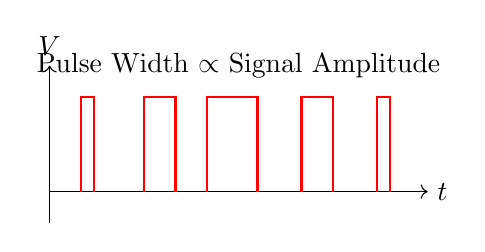
\begin{tikzpicture}[scale=0.8]
    \draw[->] (0,0) -- (6,0) node[right] {$t$};
    \draw[->] (0,-0.5) -- (0,2) node[above] {$V$};
    
    % PWM pulses
    % Narrow pulse
    \draw[thick, red] (0.5,0) -- (0.5,1.5) -- (0.7,1.5) -- (0.7,0);
    % Medium pulse
    \draw[thick, red] (1.5,0) -- (1.5,1.5) -- (2.0,1.5) -- (2.0,0);
    % Wide pulse (peak signal)
    \draw[thick, red] (2.5,0) -- (2.5,1.5) -- (3.3,1.5) -- (3.3,0);
    % Medium pulse
    \draw[thick, red] (4.0,0) -- (4.0,1.5) -- (4.5,1.5) -- (4.5,0);
    % Narrow pulse
    \draw[thick, red] (5.2,0) -- (5.2,1.5) -- (5.4,1.5) -- (5.4,0);
    
    \node at (3,2) {Pulse Width $\propto$ Signal Amplitude};
\end{tikzpicture}
\captionof{figure}{PWM Waveform}
\end{center}
\end{solutionbox}

\begin{mnemonicbox}
"PWM: Width varies, Amplitude constant"
\end{mnemonicbox}

\questionmarks{3(b) OR}{4}{What is PPM?}

\begin{solutionbox}
\textbf{Answer}:

\textbf{Pulse Position Modulation (PPM):}
PPM is a modulation technique where the position of a constant-width pulse within a prescribed time slot is varied according to the amplitude of the sampled signal.

\begin{itemize}
    \item \textbf{Constant}: Amplitude and width of pulses.
    \item \textbf{Variable}: Relative position of the pulse.
    \item \textbf{Advantage}: Requires less power than PWM (only short pulses sent).
    \item \textbf{Disadvantage}: Requires complex synchronization between Tx and Rx.
\end{itemize}

\begin{center}
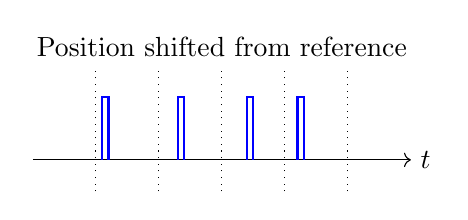
\begin{tikzpicture}[scale=0.8]
    \draw[->] (0,0) -- (6,0) node[right] {$t$};
    
    % Clock ticks / Reference moments
    \foreach \x in {1,2,3,4,5} \draw[dotted] (\x, -0.5) -- (\x, 1.5);
    
    % PPM Pulses
    % Pulse shifted slightly right
    \draw[thick, blue] (1.1,0) -- (1.1,1) -- (1.2,1) -- (1.2,0);
    % Pulse shifted more right
    \draw[thick, blue] (2.3,0) -- (2.3,1) -- (2.4,1) -- (2.4,0);
    % Pulse max shift
    \draw[thick, blue] (3.4,0) -- (3.4,1) -- (3.5,1) -- (3.5,0);
     % Pulse back to small shift
    \draw[thick, blue] (4.2,0) -- (4.2,1) -- (4.3,1) -- (4.3,0);
    
    \node at (3,1.8) {Position shifted from reference};
\end{tikzpicture}
\captionof{figure}{PPM Waveform}
\end{center}
\end{solutionbox}

\begin{mnemonicbox}
"PPM: Position Shifts, Width Fixed"
\end{mnemonicbox}

\questionmarks{3(c) OR}{7}{Describe PCM with block diagram.}

\begin{solutionbox}
\textbf{Answer}:

\begin{center}
\begin{tikzpicture}[node distance=2cm, auto, >=latex, thick, scale=0.75, transform shape]
    % PCM Transmitter
    \node [gtu block] (lpf) {LPF};
    \node [left of=lpf, node distance=2cm, align=center] (in) {Analog\\In};
    \node [gtu block, right of=lpf] (samp) {Sampler};
    \node [gtu block, right of=samp] (quant) {Quantizer};
    \node [gtu block, right of=quant] (enc) {Encoder};
    \node [right of=enc, node distance=2cm, align=center] (out) {PCM\\Out};
    
    \draw [gtu arrow] (in) -- (lpf);
    \draw [gtu arrow] (lpf) -- (samp);
    \draw [gtu arrow] (samp) -- (quant);
    \draw [gtu arrow] (quant) -- (enc);
    \draw [gtu arrow] (enc) -- (out);
\end{tikzpicture}
\captionof{figure}{PCM Transmitter}
\end{center}

\textbf{Pulse Code Modulation (PCM):}
A digital modulation technique that converts analog signals into binary form.

\textbf{Key Steps:}

\begin{center}
\captionof{table}{PCM Process}
\begin{tabulary}{\linewidth}{|L|L|}
\hline
\textbf{Step} & \textbf{Description} \\
\hline
\textbf{1. Filtering (LPF)} & Limits signal frequency to $f_m$ to prevent aliasing \\
\hline
\textbf{2. Sampling} & Discretizes signal in time ($f_s \ge 2f_m$). Output is PAM \\
\hline
\textbf{3. Quantization} & Discretizes signal in amplitude. Rounds values to nearest levels. Introduces quantization noise \\
\hline
\textbf{4. Encoding} & Converts quantized levels into binary code (0s and 1s) \\
\hline
\end{tabulary}
\end{center}

\textbf{Advantages:}
\begin{itemize}
    \item Noise immunity (digital)
    \item Possibility of storage
    \item Efficient multiplexing
\end{itemize}
\end{solutionbox}

\begin{mnemonicbox}
"FSQE: Filter, Sample, Quantize, Encode - The path to Digital"
\end{mnemonicbox}

\questionmarks{4(a)}{3}{Explain Quantization and Quantization noise.}

\begin{solutionbox}
\textbf{Answer}:

\textbf{Quantization:}
The process of approximating a continuous range of values (infinite possibilities) by a relatively small set of discrete values (finite levels).
\begin{itemize}
    \item It is a non-reversible process (lossy).
    \item Input: Sampled Signal (PAM).
    \item Output: Quantized Signal (Discrete Amplitude).
\end{itemize}

\textbf{Quantization Noise (Error):}
The difference between the actual input value and the quantized output value.
\[ \epsilon = x(t) - x_q(t) \]
\begin{itemize}
    \item Maximum error is $\pm \Delta/2$, where $\Delta$ is the step size.
    \item Random in nature, acts like additive noise.
\end{itemize}
\end{solutionbox}

\begin{mnemonicbox}
"Quantization: Rounding off values; Noise: The rounding error"
\end{mnemonicbox}

\questionmarks{4(b)}{4}{Explain Amplitude shift keying with waveforms.}

\begin{solutionbox}
\textbf{Answer}:

\textbf{Amplitude Shift Keying (ASK):}
A digital modulation technique where the amplitude of the carrier signal is switched between two levels according to the binary data.
\begin{itemize}
    \item \textbf{Logic 1}: High amplitude carrier (or simply Carrier present).
    \item \textbf{Logic 0}: Low amplitude carrier (or No carrier - OOK).
\end{itemize}

\textbf{Expression:}
\[ s(t) = \begin{cases} A_c \cos(2\pi f_c t) & \text{for Logic 1} \\ 0 & \text{for Logic 0} \end{cases} \]

\begin{center}
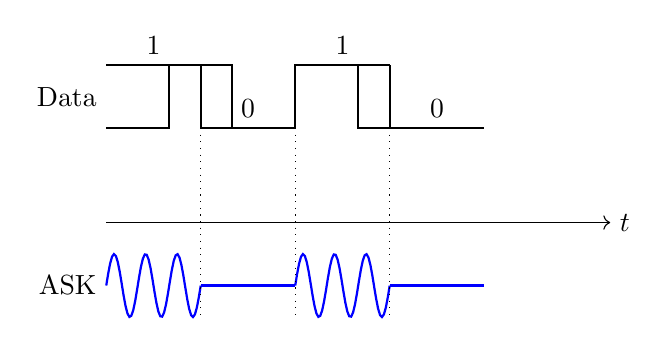
\begin{tikzpicture}[scale=0.8]
    \draw[->] (0,0) -- (8,0) node[right] {$t$};
    
    % Binary Data
    \node[left] at (0,2) {Data};
    \draw[thick] (0,1.5) -- (1,1.5) -- (1,2.5) -- (2,2.5) -- (2,1.5) -- (3,1.5) -- (3,2.5) -- (4,2.5) -- (4,1.5) -- (5,1.5) -- (5,1.5);
    % Let's draw: 1 0 1 1 0
    % Bit width = 1.5 cm
    \draw[thick] (0,2.5) -- (1.5,2.5) node[midway, above] {1}; 
    \draw[thick] (1.5,2.5) -- (1.5,1.5) -- (3,1.5) node[midway, above] {0};
    \draw[thick] (3,1.5) -- (3,2.5) -- (4.5,2.5) node[midway, above] {1};
    \draw[thick] (4.5,2.5) -- (4.5,1.5) -- (6,1.5) node[midway, above] {0};
    
    % Carrier
    \node[left] at (0,-1) {ASK};
    % Logic 1: Sine
    \draw[blue, thick, samples=50, domain=0:1.5] plot (\x, {-1 + 0.5*sin(360*2*\x)});
    % Logic 0: Zero
    \draw[blue, thick] (1.5,-1) -- (3,-1);
    % Logic 1: Sine
    \draw[blue, thick, samples=50, domain=3:4.5] plot (\x, {-1 + 0.5*sin(360*2*(\x-3))});
    % Logic 0: Zero
    \draw[blue, thick] (4.5,-1) -- (6,-1);
    
    \draw[dotted] (1.5,1.5) -- (1.5,-1.5);
    \draw[dotted] (3,1.5) -- (3,-1.5);
    \draw[dotted] (4.5,1.5) -- (4.5,-1.5);
\end{tikzpicture}
\captionof{figure}{ASK Waveforms}
\end{center}
\end{solutionbox}

\begin{mnemonicbox}
"ASK: Amplitude Switched Keying - Carrier On/Off"
\end{mnemonicbox}

\questionmarks{4(c)}{7}{Compare ASK, FSK and PSK techniques.}

\begin{solutionbox}
\textbf{Answer}:

\begin{center}
\captionof{table}{Comparison of Digital Modulation Techniques}
\begin{tabulary}{\linewidth}{|L|L|L|L|}
\hline
\textbf{Parameter} & \textbf{ASK} & \textbf{FSK} & \textbf{PSK} \\
\hline
\textbf{Definition} & Amplitude varies with data & Frequency varies with data & Phase varies with data \\
\hline
\textbf{Bandwidth} & Approx $2 \times R_b$ & Large, $> 2 \times R_b$ & Approx $2 \times R_b$ \\
\hline
\textbf{Noise Immunity} & Low (Affected by amplitude noise) & High (Envelope constant) & High (Envelope constant) \\
\hline
\textbf{Bit Error Rate} & High & Medium & Low (Performance best) \\
\hline
\textbf{Complexity} & Simple & Medium & Complex \\
\hline
\textbf{Applications} & Optical fiber, low speed data & Modems, Radio & WiFi, Satellite, Bluetooth \\
\hline
\end{tabulary}
\end{center}
\end{solutionbox}

\begin{mnemonicbox}
"Comparison: FSK/PSK beat ASK in noise; PSK best performance"
\end{mnemonicbox}

\questionmarks{4(a) OR}{3}{Explain Frequency shift keying with waveforms.}

\begin{solutionbox}
\textbf{Answer}:

\textbf{Frequency Shift Keying (FSK):}
A digital modulation technique where frequency of the carrier is shifted between two values.
\begin{itemize}
    \item \textbf{Logic 1}: High Frequency Carrier ($f_1$).
    \item \textbf{Logic 0}: Low Frequency Carrier ($f_2$).
    \item \textbf{Amplitude}: Remains constant.
\end{itemize}

\begin{center}
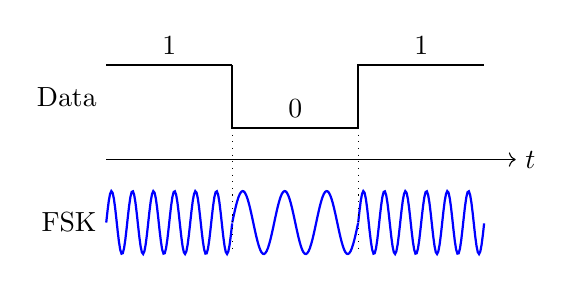
\begin{tikzpicture}[scale=0.8]
    \draw[->] (0,0) -- (6.5,0) node[right] {$t$};
    
    % Data: 1 0 1
    \draw[thick] (0,1.5) -- (2,1.5) node[midway, above] {1};
    \draw[thick] (2,1.5) -- (2,0.5) -- (4,0.5) node[midway, above] {0};
    \draw[thick] (4,0.5) -- (4,1.5) -- (6,1.5) node[midway, above] {1};
    
    \node[left] at (0,1) {Data};
    \node[left] at (0,-1) {FSK};
    
    % FSK Waveform
    % Logic 1: High Freq 
    \draw[blue, thick, samples=100, domain=0:2] plot (\x, {-1 + 0.5*sin(360*3*\x)});
    % Logic 0: Low Freq
    \draw[blue, thick, samples=100, domain=2:4] plot (\x, {-1 + 0.5*sin(360*1.5*\x)});
    % Logic 1: High Freq
    \draw[blue, thick, samples=100, domain=4:6] plot (\x, {-1 + 0.5*sin(360*3*\x)});
    
    \draw[dotted] (2,0.5) -- (2,-1.5);
    \draw[dotted] (4,0.5) -- (4,-1.5);
\end{tikzpicture}
\captionof{figure}{FSK Waveforms}
\end{center}
\end{solutionbox}

\begin{mnemonicbox}
"FSK: Frequency Switched Keying - High/Low tones"
\end{mnemonicbox}

\questionmarks{4(b) OR}{4}{Explain Phase shift keying with waveforms.}

\begin{solutionbox}
\textbf{Answer}:

\textbf{Phase Shift Keying (PSK):}
A digital modulation technique where phase of the carrier is shifted (usually by 180 degrees) according to binary data.
\begin{itemize}
    \item \textbf{Logic 1}: Carrier with $0^\circ$ phase.
    \item \textbf{Logic 0}: Carrier with $180^\circ$ phase.
    \item \textbf{Amplitude \& Frequency}: Constant.
\end{itemize}

\begin{center}
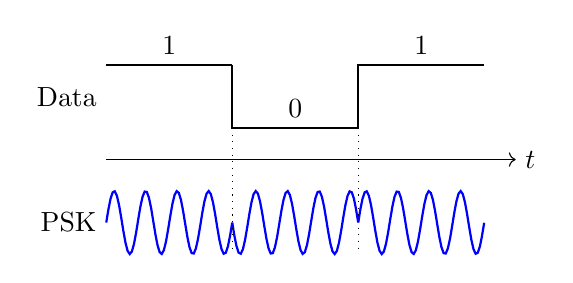
\begin{tikzpicture}[scale=0.8]
    \draw[->] (0,0) -- (6.5,0) node[right] {$t$};
    
    % Data: 1 0 1
    \draw[thick] (0,1.5) -- (2,1.5) node[midway, above] {1};
    \draw[thick] (2,1.5) -- (2,0.5) -- (4,0.5) node[midway, above] {0};
    \draw[thick] (4,0.5) -- (4,1.5) -- (6,1.5) node[midway, above] {1};
    
    \node[left] at (0,1) {Data};
    \node[left] at (0,-1) {PSK};
    
    % PSK Waveform
    % Logic 1: Sine
    \draw[blue, thick, samples=60, domain=0:2] plot (\x, {-1 + 0.5*sin(360*2*\x)});
    % Logic 0: -Sine (180 shift)
    \draw[blue, thick, samples=60, domain=2:4] plot (\x, {-1 - 0.5*sin(360*2*\x)});
    % Logic 1: Sine
    \draw[blue, thick, samples=60, domain=4:6] plot (\x, {-1 + 0.5*sin(360*2*\x)});
    
    \draw[dotted] (2,0.5) -- (2,-1.5);
    \draw[dotted] (4,0.5) -- (4,-1.5);
\end{tikzpicture}
\captionof{figure}{PSK Waveforms}
\end{center}
\end{solutionbox}

\begin{mnemonicbox}
"PSK: Phase Switched - 0 to 180 flip"
\end{mnemonicbox}

\questionmarks{4(c) OR}{7}{Explain DPCM with suitable block diagram.}

\begin{solutionbox}
\textbf{Answer}:

\textbf{Differential Pulse Code Modulation (DPCM):}
A technique where, instead of transmitting the absolute sample value, the *difference* between consecutive samples (or predicted and actual sample) is quantized and transmitted.
\begin{itemize}
    \item \textbf{Goal}: Takes advantage of correlation between adjacent samples to reduce bandwidth.
    \item \textbf{Process}: $e[n] = x[n] - \hat{x}[n]$, then $e[n]$ is quantized and encoded.
\end{itemize}

\begin{center}
\begin{tikzpicture}[node distance=2cm, auto, >=latex, thick, scale=0.7, transform shape]
    % Transmitter
    \node (in) {Input $x[n]$};
    \node [draw, circle, right of=in, inner sep=1pt] (sub) {$\Sigma$};
    \node [right of=sub, node distance=1.5cm] (e) {$e[n]$};
    \node [gtu block, right of=sub, node distance=2.5cm] (quant) {Quantizer};
    \node [gtu block, right of=quant, node distance=2.5cm] (enc) {Encoder};
    \node [right of=enc, node distance=2cm] (out) {DPCM Out};
    
    % Feedback Path
    \node [draw, circle, below of=quant, node distance=2cm, inner sep=1pt] (add) {$\Sigma$};
    \node [gtu block, left of=add, node distance=2.5cm] (pred) {Prediction\\Filter};
    \node [below of=quant, node distance=1.2cm] (eq) {$e_q[n]$};
    
    % Connections
    \draw [gtu arrow] (in) -- (sub);
    \draw [gtu arrow] (sub) -- (quant);
    \draw [gtu arrow] (quant) -- (enc);
    \draw [gtu arrow] (enc) -- (out);
    
    \draw [gtu arrow] (quant) -- (add);
    \draw [gtu arrow] (add) -- (pred);
    \draw [gtu arrow] (pred) -| (sub) node[pos=0.9, left] {-};
    \draw [gtu arrow] (pred) -| (add) node[pos=0.9, left] {+};
    
    \node[left] at (sub.west) {+};
\end{tikzpicture}
\captionof{figure}{DPCM Transmitter Block Diagram}
\end{center}

\textbf{Advantages:}
\begin{itemize}
    \item Reduced bandwidth requirement compared to PCM.
    \item Better SNR for same bit rate.
\end{itemize}
\end{solutionbox}

\begin{mnemonicbox}
"DPCM: Difference Encoded - Send only the change"
\end{mnemonicbox}

\questionmarks{5(a)}{3}{Compare PCM and DM}

\begin{solutionbox}
\textbf{Answer}:

\begin{center}
\captionof{table}{Comparison of PCM and DM}
\begin{tabulary}{\linewidth}{|L|L|L|}
\hline
\textbf{Parameter} & \textbf{PCM} & \textbf{DM (Delta Modulation)} \\
\hline
\textbf{Bit Rate} & Higher (multiple bits per sample) & Lower (1 bit per sample) \\
\hline
\textbf{Circuit Complexity} & More complex & Simpler \\
\hline
\textbf{Signal Quality} & Better & Lower, suffers from slope overload \& granular noise \\
\hline
\textbf{Bandwidth} & Wider & Narrower \\
\hline
\textbf{Sampling Rate} & At least $2f_m$ & Much higher than $2f_m$ \\
\hline
\end{tabulary}
\end{center}
\end{solutionbox}

\begin{mnemonicbox}
"BCSBS: Bit rate, Complexity, Signal quality, Bandwidth, Sampling"
\end{mnemonicbox}

\questionmarks{5(b)}{4}{Define: (A) Antenna (B) Radiation pattern (C) Directivity and (D) Polarization}

\begin{solutionbox}
\textbf{Answer}:

\begin{center}
\captionof{table}{Antenna Terminology}
\begin{tabulary}{\linewidth}{|L|L|}
\hline
\textbf{Term} & \textbf{Definition} \\
\hline
\textbf{Antenna} & Device that converts electrical signals into electromagnetic waves and vice versa \\
\hline
\textbf{Radiation Pattern} & Graphical representation of radiation properties of antenna as function of space coordinates \\
\hline
\textbf{Directivity} & Ratio of radiation intensity in a given direction to average radiation intensity \\
\hline
\textbf{Polarization} & Orientation of electric field vector of electromagnetic wave radiated by antenna \\
\hline
\end{tabulary}
\end{center}

\begin{center}
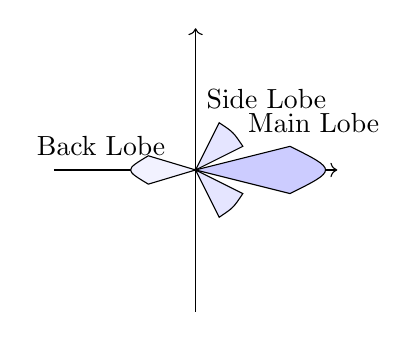
\begin{tikzpicture}[scale=0.6]
    % Coordinates
    \draw[->] (-3,0) -- (3,0);
    \draw[->] (0,-3) -- (0,3);
    
    % Main Lobe
    \draw[fill=blue!20] (0,0) -- (2,0.5) .. controls (3,0) .. (2,-0.5) -- cycle;
    
    % Side Lobes
    \draw[fill=blue!10] (0,0) -- (0.5,1) .. controls (0.8,0.8) .. (1,0.5) -- cycle;
    \draw[fill=blue!10] (0,0) -- (0.5,-1) .. controls (0.8,-0.8) .. (1,-0.5) -- cycle;
    
    % Back Lobe
    \draw[fill=blue!5] (0,0) -- (-1,0.3) .. controls (-1.5,0) .. (-1,-0.3) -- cycle;
    
    \node at (2.5,1) {Main Lobe};
    \node at (1.5,1.5) {Side Lobe};
    \node at (-2,0.5) {Back Lobe};
\end{tikzpicture}
\captionof{figure}{Radiation Pattern}
\end{center}
\end{solutionbox}

\begin{mnemonicbox}
"ARDP: Antennas Radiate with Directivity and Polarization"
\end{mnemonicbox}

\questionmarks{5(c)}{7}{Write brief note on (A) smart antenna (B) parabolic reflector antenna}

\begin{solutionbox}
\textbf{Answer}:

\subsubsection*{(A) Smart Antenna}
\begin{center}
\captionof{table}{Smart Antenna Characteristics}
\begin{tabulary}{\linewidth}{|L|L|}
\hline
\textbf{Feature} & \textbf{Description} \\
\hline
\textbf{Definition} & Antenna array with signal processing capability to adapt to changing conditions \\
\hline
\textbf{Types} & Switched beam, Adaptive array \\
\hline
\textbf{Benefits} & Increased range/coverage, interference reduction, capacity improvement \\
\hline
\textbf{Applications} & Mobile communications, 5G networks, WiMAX, military systems \\
\hline
\end{tabulary}
\end{center}

\textbf{Block Diagram:}
\begin{center}
\begin{tikzpicture}[node distance=2.5cm, auto, >=latex, thick]
    \node [gtu block] (sp) {Signal\\Processor};
    \node [gtu block, left of=sp, node distance=3cm] (fe) {RF Front\\End};
    \node [left of=fe, node distance=2.5cm] (ant) {Array};
    \node [gtu block, right of=sp, node distance=3cm] (bf) {Beam\\Forming};
    
    \draw [thick] (ant) -- (fe);
    \foreach \y in {0.3, 0.1, -0.1, -0.3} \draw (ant.east) -- (fe.west); % Multiple lines
    
    \draw [gtu arrow] (fe) -- (sp);
    \draw [gtu arrow] (sp) -- (bf);
    \draw [gtu arrow] (bf) -- (fe); % Feedback
\end{tikzpicture}
\captionof{figure}{Smart Antenna System}
\end{center}

\subsubsection*{(B) Parabolic Reflector Antenna}
\begin{center}
\captionof{table}{Parabolic Reflector Characteristics}
\begin{tabulary}{\linewidth}{|L|L|}
\hline
\textbf{Feature} & \textbf{Description} \\
\hline
\textbf{Structure} & Feed antenna at focal point with parabolic reflecting surface \\
\hline
\textbf{Operation} & Focuses parallel incoming waves to focal point or radiates from focal point into parallel beams \\
\hline
\textbf{Gain} & Very high directivity and gain \\
\hline
\textbf{Applications} & Satellite communication, radio astronomy, radar systems \\
\hline
\end{tabulary}
\end{center}

\begin{center}
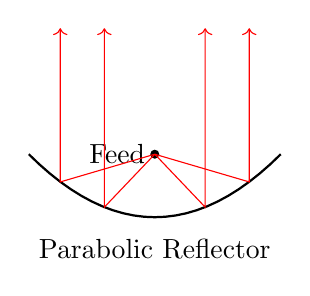
\begin{tikzpicture}[scale=0.8]
    % Parabola
    \draw[thick, domain=-2:2] plot (\x, {0.25*\x*\x});
    
    % Focus
    \node[draw, circle, fill=black, inner sep=1pt] (focus) at (0,1) {};
    \node[left] at (focus) {Feed};
    
    % Rays
    \draw[->, red] (0,1) -- (1.5, 0.56) -- (1.5, 3);
    \draw[->, red] (0,1) -- (-1.5, 0.56) -- (-1.5, 3);
    \draw[->, red] (0,1) -- (0.8, 0.16) -- (0.8, 3);
    \draw[->, red] (0,1) -- (-0.8, 0.16) -- (-0.8, 3);
    
    \node at (0,-0.5) {Parabolic Reflector};
\end{tikzpicture}
\captionof{figure}{Parabolic Reflector}
\end{center}
\end{solutionbox}

\begin{mnemonicbox}
"PFHS: Parabolic Focus gives High Signal strength"
\end{mnemonicbox}

\questionmarks{5(a) OR}{3}{Write a short note on Microstrip antenna}

\begin{solutionbox}
\textbf{Answer}:

\begin{center}
\captionof{table}{Microstrip Antenna Characteristics}
\begin{tabulary}{\linewidth}{|L|L|}
\hline
\textbf{Feature} & \textbf{Description} \\
\hline
\textbf{Structure} & Conductive patch on dielectric substrate with ground plane \\
\hline
\textbf{Shape} & Rectangular, circular, elliptical, triangular patches \\
\hline
\textbf{Size} & Typically $\lambda/2$ in length, very thin ($h \ll \lambda$) \\
\hline
\textbf{Advantages} & Low profile, lightweight, low cost, easy fabrication, compatible with PCB technology \\
\hline
\textbf{Disadvantages} & Low efficiency, narrow bandwidth, low power handling \\
\hline
\end{tabulary}
\end{center}

\begin{center}
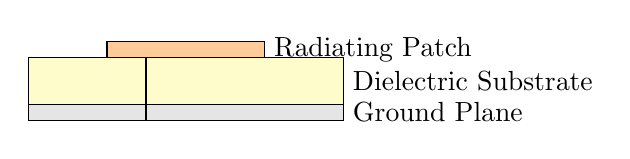
\begin{tikzpicture}[scale=1]
    % Ground Plane
    \draw[fill=gray!20] (0,0) rectangle (4,0.2);
    \node[right] at (4,0.1) {Ground Plane};
    
    % Substrate
    \draw[fill=yellow!20] (0,0.2) rectangle (4,0.8);
    \node[right] at (4,0.5) {Dielectric Substrate};
    
    % Patch
    \draw[fill=orange!40] (1,0.8) rectangle (3,1.0);
    \node[right] at (3,0.9) {Radiating Patch};
    
    % Feed line
    \draw[thick] (1.5, 0) -- (1.5, 0.8); % Probe feed representation
\end{tikzpicture}
\captionof{figure}{Microstrip Patch Antenna (Side View)}
\end{center}
\end{solutionbox}

\begin{mnemonicbox}
"PDGF: Patch on Dielectric with Ground plane gives Flat profile"
\end{mnemonicbox}

\questionmarks{5(b) OR}{4}{Explain EM wave spectrum, its Frequency ranges and its applications.}

\begin{solutionbox}
\textbf{Answer}:

\begin{center}
\captionof{table}{EM Wave Spectrum and Applications}
\begin{tabulary}{\linewidth}{|L|L|L|L|}
\hline
\textbf{Band} & \textbf{Frequency Range} & \textbf{Wavelength} & \textbf{Applications} \\
\hline
\textbf{ELF} & 3 Hz - 30 Hz & 100 Mm & Submarine comm. \\
\hline
\textbf{VLF} & 3 kHz - 30 kHz & 10-100 km & Navigation \\
\hline
\textbf{LF} & 30-300 kHz & 1-10 km & AM radio \\
\hline
\textbf{MF} & 300 kHz - 3 MHz & 100m - 1 km & AM broadcast \\
\hline
\textbf{HF} & 3-30 MHz & 10-100 m & Shortwave \\
\hline
\textbf{VHF} & 30-300 MHz & 1-10 m & FM, TV \\
\hline
\textbf{UHF} & 300 MHz - 3 GHz & 10cm - 1m & Mobile, WiFi \\
\hline
\textbf{SHF} & 3-30 GHz & 1-10 cm & Satellite, Radar \\
\hline
\textbf{EHF} & 30-300 GHz & 1-10 mm & Radio astronomy \\
\hline
\textbf{Visible} & 400-800 THz & 380-750 nm & Optical comm. \\
\hline
\end{tabulary}
\end{center}

\begin{center}
\begin{tikzpicture}[scale=0.9, transform shape]
    \node [gtu block, fill=blue!10] (radio) {Radio};
    \node [gtu block, right of=radio, node distance=2.5cm, fill=blue!20] (micro) {Microwave};
    \node [gtu block, right of=micro, node distance=2.5cm, fill=orange!20] (ir) {IR};
    \node [gtu block, right of=ir, node distance=2.5cm, fill=yellow!20] (vis) {Visible};
    \node [gtu block, right of=vis, node distance=2.5cm, fill=purple!20] (uv) {UV};
    
    \draw [gtu arrow] (radio) -- (micro);
    \draw [gtu arrow] (micro) -- (ir);
    \draw [gtu arrow] (ir) -- (vis);
    \draw [gtu arrow] (vis) -- (uv);
    
    \node [below of=radio, node distance=1cm] {Low $f$};
    \node [below of=uv, node distance=1cm] {High $f$};
\end{tikzpicture}
\captionof{figure}{EM Spectrum Increasing Frequency}
\end{center}
\end{solutionbox}

\begin{mnemonicbox}
"RVMIXG: Radio, Visible, Microwave, Infrared, X-ray, Gamma"
\end{mnemonicbox}

\questionmarks{5(c) OR}{7}{Write brief note on (A) Space Wave Propagation (B) Ground Wave Propagation.}

\begin{solutionbox}
\textbf{Answer}:

\subsubsection*{(A) Space Wave Propagation}
\begin{center}
\captionof{table}{Space Wave Propagation Characteristics}
\begin{tabulary}{\linewidth}{|L|L|}
\hline
\textbf{Feature} & \textbf{Description} \\
\hline
\textbf{Definition} & Direct wave propagation through space, including line-of-sight (LOS) and reflected waves \\
\hline
\textbf{Frequency Range} & VHF and above ($>30$ MHz) \\
\hline
\textbf{Distance} & Limited by horizon, typically 50-80 km \\
\hline
\textbf{Types} & Direct wave, Ground reflected wave \\
\hline
\textbf{Applications} & TV broadcasting, microwave links, satellite communication \\
\hline
\end{tabulary}
\end{center}

\begin{center}
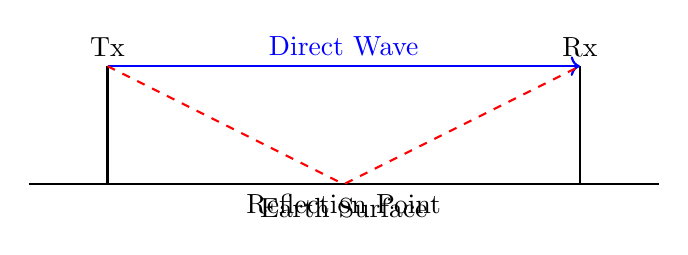
\begin{tikzpicture}[scale=1]
    % Ground
    \draw[thick] (-4,0) -- (4,0);
    \node at (0,-0.3) {Earth Surface};
    
    % Tx Tower
    \draw[thick] (-3,0) -- (-3,1.5);
    \node[above] at (-3,1.5) {Tx};
    
    % Rx Tower
    \draw[thick] (3,0) -- (3,1.5);
    \node[above] at (3,1.5) {Rx};
    
    % Direct Wave
    \draw[->, blue, thick] (-3,1.5) -- node[above] {Direct Wave} (3,1.5);
    
    % Reflected Wave
    \draw[dashed, red, thick] (-3,1.5) -- (0,0) -- (3,1.5);
    \node[below] at (0,0) {Reflection Point};
\end{tikzpicture}
\captionof{figure}{Space Wave Propagation}
\end{center}

\subsubsection*{(B) Ground Wave Propagation}
\begin{center}
\captionof{table}{Ground Wave Characteristics}
\begin{tabulary}{\linewidth}{|L|L|}
\hline
\textbf{Feature} & \textbf{Description} \\
\hline
\textbf{Definition} & Wave propagation along Earth's surface, follows curvature of Earth \\
\hline
\textbf{Frequency Range} & LF, MF (up to 2 MHz) \\
\hline
\textbf{Distance} & Up to 1000 km depending on frequency and power \\
\hline
\textbf{Mechanism} & Vertically polarized wave induces current in conductive Earth surface \\
\hline
\textbf{Applications} & AM radio broadcasting, maritime communication \\
\hline
\end{tabulary}
\end{center}

\begin{center}
\begin{tikzpicture}[scale=1]
    % Curved Earth
    \draw[thick] (-4,0) to[bend left=10] (4,0);
    \node at (0,-1) {Earth Curvature};
    
    % Tx
    \draw[thick] (-3.5, -0.2) -- (-3.5, 1);
    \node[above] at (-3.5, 1) {Tx};
    
    % Rx
    \draw[thick] (3.5, -0.2) -- (3.5, 1);
    \node[above] at (3.5, 1) {Rx};
    
    % Surface Wave
    \draw[->, blue, thick, snake=coil, segment aspect=0] (-3.5, 0.5) to[bend left=15] node[above] {Ground Wave} (3.5, 0.5);
    
\end{tikzpicture}
\captionof{figure}{Ground Wave Propagation}
\end{center}
\end{solutionbox}

\begin{mnemonicbox}
"SHGM: Space waves go High, Ground waves hug Medium surface"
\end{mnemonicbox}

\end{document}

